\documentclass[11pt]{standalone}
\usepackage{amssymb}
\usepackage{amsmath}
\usepackage[no-math]{fontspec}
\usepackage{unicode-math}
\setmainfont{Libertinus Sans}
\setsansfont{Libertinus Sans}
\setmathfont{Libertinus Math}
\usepackage{pgf,xcolor}
\usepackage{tikz}
\usetikzlibrary{arrows.meta, backgrounds, calc}
\usepackage{pgfplots}
\pgfplotsset{compat=newest}
\usepackage{pifont}

\definecolor{my_darkgray}{HTML}{484949}
\definecolor{my_lightgray}{HTML}{F3F4F4}
\definecolor{my_darkblue}{HTML}{005A94}
\definecolor{my_lightblue}{HTML}{CCDEE9}
\definecolor{my_yellow}{HTML}{FFEC7F}
\definecolor{my_red}{HTML}{E60000}
\definecolor{my_orange}{HTML}{E87846}

\begin{document}
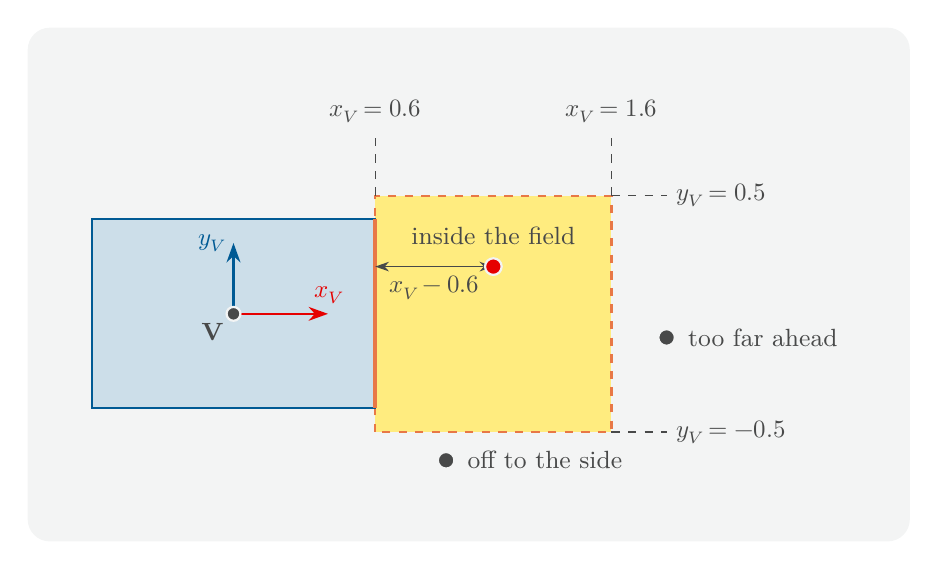
\begin{tikzpicture}[
    show background rectangle,
    background rectangle/.style={fill=my_lightgray, rounded corners=8pt},
    inner frame sep=0.8cm,
    achse/.style={thick, -{Stealth[length=7pt, width=5pt]}},
    bemassung/.style={draw=my_darkgray, thin, {Stealth[length=5pt, width=3.5pt]}-{Stealth[length=5pt, width=3.5pt]}},
    hilfslinie/.style={draw=my_darkgray, thin, dashed},
    annotation/.style={draw=my_darkgray, thick, -{Stealth[length=7pt, width=5pt]}}
]

    % Schutzfeld im Fahrzeugkoordinatensystem, Maßstab 1 m = 3 cm.
    % Fahrzeug 1.2 m x 0.8 m, Schutzfeld x_V von 0.6 bis 1.6 m,
    % y_V von -0.5 bis 0.5 m. Die drei Messpunkte sind frei gewählt.

    % Schutzfeld
    \draw[fill=my_yellow, draw=my_orange, thick, dashed] (1.8,-1.5) rectangle (4.8,1.5);

    % Fahrzeug: Umriss hellblau, Vorderkante orange
    \draw[fill=my_lightblue, draw=my_darkblue, thick] (-1.8,-1.2) rectangle (1.8,1.2);
    \draw[draw=my_orange, ultra thick] (1.8,-1.2) -- (1.8,1.2);

    % Fahrzeugkoordinatensystem F
    \coordinate (F) at (0,0);
    \draw[achse, draw=my_red] (F) -- (1.2,0)
        node[anchor=south, font=\small, text=my_red] {$x_V$};
    \draw[achse, draw=my_darkblue] (F) -- (0,0.9)
        node[anchor=east, font=\small, text=my_darkblue] {$y_V$};
    \node[font=\small\bfseries, text=my_darkgray, anchor=north east] at (F) {V};
    \draw[fill=my_darkgray, draw=my_lightgray, thick] (F) circle (2.5pt);

    % Grenzen des Schutzfelds in Fahrtrichtung
    \draw[hilfslinie] (1.8,1.5) -- (1.8,2.3);
    \draw[hilfslinie] (4.8,1.5) -- (4.8,2.3);
    \node[font=\small, text=my_darkgray, anchor=south] at (1.8,2.3) {$x_V = 0.6$};
    \node[font=\small, text=my_darkgray, anchor=south] at (4.8,2.3) {$x_V = 1.6$};

    % Grenzen des Schutzfelds quer zur Fahrtrichtung
    \draw[hilfslinie] (4.8,1.5) -- (5.5,1.5);
    \draw[hilfslinie] (4.8,-1.5) -- (5.5,-1.5);
    \node[font=\small, text=my_darkgray, anchor=west] at (5.5,1.5) {$y_V = 0.5$};
    \node[font=\small, text=my_darkgray, anchor=west] at (5.5,-1.5) {$y_V = -0.5$};

    % Messpunkt im Schutzfeld mit seinem Längsabstand zur Vorderkante
    \coordinate (P1) at (3.3,0.6);
    \draw[bemassung] (1.8,0.6) -- (P1)
        node[midway, anchor=north, font=\small, text=my_darkgray] {$x_V - 0.6$};
    \draw[fill=my_red, draw=my_lightgray, thick] (P1) circle (3pt);
    \node[font=\small, text=my_darkgray, anchor=south] at (3.3,0.75) {inside the field};

    % Messpunkt zu weit vorne
    \coordinate (P2) at (5.5,-0.3);
    \draw[fill=my_darkgray, draw=my_lightgray, thick] (P2) circle (3pt);
    \node[font=\small, text=my_darkgray, anchor=west] at (5.65,-0.3) {too far ahead};

    % Messpunkt seitlich neben dem Schutzfeld
    \coordinate (P3) at (2.7,-1.86);
    \draw[fill=my_darkgray, draw=my_lightgray, thick] (P3) circle (3pt);
    \node[font=\small, text=my_darkgray, anchor=west] at (2.85,-1.86) {off to the side};

\end{tikzpicture}
\end{document}
